\documentclass[10pt]{article}
\usepackage[margin=0.65in]{geometry}\usepackage[T1]{fontenc}\usepackage{graphicx}
\begin{document}\section*{One bounded private runtime assembly}
The worker completed its COPY-only assembly and retained the resulting image and disk. The launcher then failed while parsing its loop-device cleanup query. This report preserves the original unresolved disposition and the separate observations used to investigate it.
\begin{center}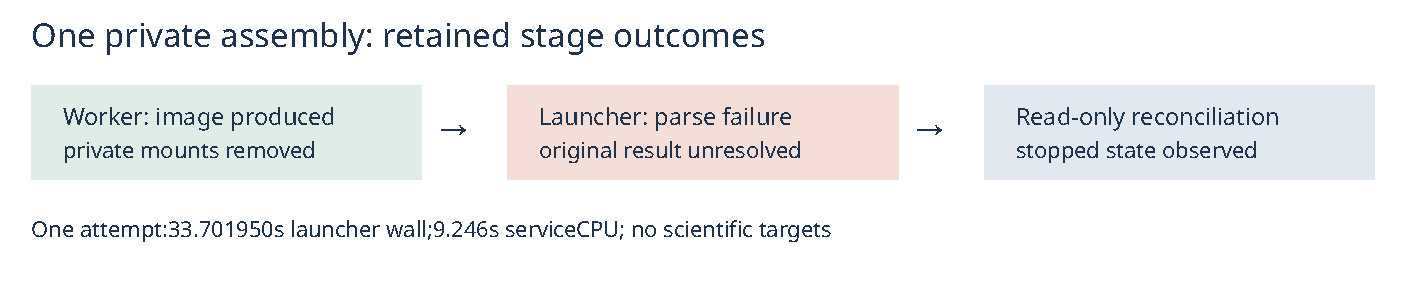
\includegraphics[width=\linewidth]{diagram.pdf}\end{center}
\textbf{Exact attempt.} Published revision2b037c3096; owner2d885f49-d570-4a8b-990e-7ea14ee9ea80. One600-second allowance,2CPU quota,2GiB RAM and4GiB disk. The command exited1 after33.701950079seconds. Systemd journal reports9.246CPU-seconds. These are separate clocks, not a speed comparison.

\textbf{Produced artifacts.} The worker receipt identifies image sha256:3a2bb98af4743c88... and disk digest 2a47f831c97c9aab... (full hashes in native-worker-result.json). It records private mounts removed and endpoint not live. Native receipt bytes and completed service-state snapshot remain preserved.

\textbf{Failure and observation.} The original losetup JSON query lacked explicit list mode and returned exit0 with empty output on this host. JSON parsing failed. A separate read-only query with explicit list mode returns a valid empty loopdevices list. The service is now not-found, inactive/dead, with empty ControlGroup. No build was repeated and no qualification or scientific target ran. The independently reviewed read-only checker returned assembled-stopped-observed with two matching stopped/empty observations. Disk custody and native receipt bytes were unchanged; the worker disk digest is inherited, not freshly rehashed. The original receipt remains unchanged.

\textbf{Accounting and custody.} Retain the conservative1200-worker-second debit and USD1 attempt allocation. The separate USD55 shared-cost margin remains recorded. The4GiB backing file stays at its native path under the allocation through November4 at06:00UTC; its hash, inode, device and timestamps are in the native worker receipt. No implicit deletion is authorized.

\textbf{Review artifacts.} publication.json, launch-start.json, launch-completion.json, native receipts, journal.stdout and read-only-observations.json bind the result. result.json is the standardized summary. The diagram is used because there is one attempt and no comparative sample.
\end{document}